% !Mode:: "TeX:UTF-8"
% !TEX root = ..\main.tex
\chapter{冠状动脉切割几种方法的实质和实现}
\section{水平集方法}
水平集方法的原理和实现
\section{聚类方法}
聚类方法的原理和实现
\section{snake方法}
\subsection{snake模型}
1987年Kass等人提出动态轮廓模型\cite{kass1988snakes},这个模型的提出主要是为了找数字图像中的
凸出轮廓,像物体的边界。动态轮廓模型被用于图像的切割和理解,也可以用于动态图像数据
的分析,例如运动跟踪。Kass等人\cite{kass1988snakes}的这篇文章给出了动态轮廓模型的基础,描述了蛇模型的基础等式。其他变种的蛇模型都是以
Kass的这个蛇模型为基础的。他的这个蛇模型也被称为经典蛇模型。
\subsubsection{蛇模型的参数化表示}
蛇模型被定义为能量最小化的样条,它的能量取决于它的形状和它在图像中的位置。蛇模型刚开始的时候形状和在图像中的
位置可以是任意的,然后演化成目标形状,移动到想要的位置和物体的边界或者边缘对齐。蛇模型的演化和移动受到最小化能量的内在趋势激活。当蛇模型和图像中目标物体的边界对齐时,它的能量达到局部最小值。

在\cite{kass1988snakes}中,蛇模型的参数化形式如下:
\begin{align}\label{eq:base_snake_parameter_representation}
	v(s) = [x(s),y(s)],s \in [0,1]
\end{align}

在上面公式中,$x(s),y(s)$是轮廓上各个点的$x,y$坐标,$s$代表弧长,$s$的范围是$[0,1]$。

曲线上每一点的移动,都是为了最小化蛇模型能量函数,它由三个能量成分组成:
\begin{align}\label{eq:base_snake_calculative_representation}
	E = \int_0^1E_{int}(v(s))+E_{image}(v(s))+E_{con}(v(s)) ds
\end{align}

在上面公式中,$E_{int}$代表内在能量,$E_{image}$代表图像能量,$E_{con}$代表外部能量。

\subsubsection{内部能量}
蛇模型每一点的内部能量按照如下方式定义
\begin{align}\label{eq:base_snake_calculative_internal_representation}
	E_{int} = \frac{1}{2}(\alpha|v^{'}(s)|^{2}+\beta|v^{''}(s)|^{2})
\end{align}

在上面公式中$v^{'}(s)=\frac{dv(s)}{ds}$定义了某点沿着切线方向的形变;公式$v^{''}(s)=\frac{d^{2}v(s)}{ds^{2}}$中的定义了某点处曲率的形变。
$\alpha,\beta$是权重系数,各自控制蛇模型的伸缩和弯曲。$\alpha$是伸缩系数,$\beta$是强直系数。


我们很容易找到一种物质用作类比蛇模型,它就是橡皮筋,橡皮筋既能拉长也能弯曲。蛇模型的内部能量是所有点按照公式\eqref{eq:base_snake_calculative_internal_representation}
求出的能量的积分,为了方便解释内部能量又被分成两部分。\eqref{eq:base_snake_calculative_internal_representation}的第一部分被称作伸缩能量,第二部分称作弯曲能量。对它们各自进行
积分得到整个蛇模型的伸缩能量和弯曲能量。

\begin{align}\label{eq:base_snake_calculative_internal_elastic_representation}
	E_{elastic} = \frac{1}{2}\int\alpha(s)|v^{'}(s)|^{2}ds
\end{align}

\begin{align}\label{eq:base_snake_calculative_internal_bending_representation}
	E_{elastic} = \frac{1}{2}\int\beta(s)|v^{''}(s)|^{2}ds
\end{align}

通常来说,$\alpha(s)$和$\beta(s)$在蛇模型中对每一点来说是一样的,就是可以被当作常量。可以用\eqref{eq:base_snake_calculative_internal_elastic_representation}
和\eqref{eq:base_snake_calculative_internal_bending_representation}的最小值解释蛇模型的形变趋势。

(1)伸缩力量:

公式\eqref{eq:base_snake_calculative_internal_elastic_representation}达到最小值,当$v^{'}(s)=0$或者$v(s)=const$,也就是蛇模型的每一点在同一位置。换句话
说,换句话说伸缩力量使得蛇模型变成一个点。

(2)弯曲力量:

公式\eqref{eq:base_snake_calculative_internal_bending_representation}达到最小值,当$v^{''}=0$,这也意味着:
\begin{align}\label{eq:simple_vs_function}
	v(s) = cs
\end{align}

公式\eqref{eq:simple_vs_function}是线性等式。从几何上来说,$v^{''}(s)=0$代表着蛇模型的曲率。所以蛇模型在曲率值高的地方尽量演变成一条直线或者磨平尖角。

\begin{figure}[htbp]
	\centering
	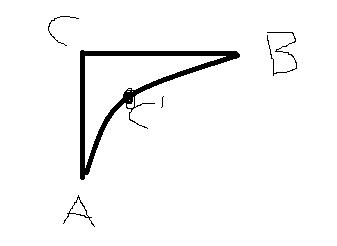
\includegraphics[width=0.5\linewidth]{snakesSmoothOverSharpCorner.png}
	\caption{蛇模型尖角处平滑}\label{fig:snakesSmoothOverSharpCorner}
\end{figure}

在图\ref{fig:snakesSmoothOverSharpCorner}中,点$C$的曲率比$C^{'}$的高。我们假设$AC^{'}B$的半径和$ACB$的半径一样。因为$AC+BC$的弧长比$AC^{'}B$长,
所以点$C$的曲率比点$C^{'}$的曲率高。


snake方法的原理和实现

学位论文基本结构包括前置部份、主体部份和结尾部份\footnote{测试脚注另起一章编号的变化}。
\section{前置部分包括}
\begin{enumerate}
	\item 封面
	\item 题名页
	\item 英文题名页(硕士可省略)
	\item 独创性声明(知识产权声明?)
	\item 勘误表(可根据需要)
	\item 致谢
	\item 序言或前沿(可根据需要)
	\item 摘要页
	\item 目次页
	\item 插图和附表清单(可根据需要)
	\item 缩写、符号清单、术语表(可根据需要)
\end{enumerate}
\section{主体部分}
\begin{enumerate}
	\item 引言(绪论)
	\item 正文
	\item 结论
\end{enumerate}
\section{结尾部分}
\begin{enumerate}
	\item 参考文献
	\item 附录(可根据需要)
	\item 索引(根据需要)
	\item 作者简历及在学期间所取得的科研成果
	\item 封底
\end{enumerate}
\chapter{基于hessian过滤器多尺度的搜索方法}
\section{原理介绍}
具体讲一下hessian矩阵的数学原理
\begin{table}[htb]
	\caption{文章字体设置效果}
	\label{tab:文章字体设置效果}
	\begin{center}
		\begin{tabular}{ccc}
			\toprule
					& 英文字体 & 中文字体  \\
			\midrule
			正文字体 & I can eat glass, it doesn't hurt me. & 我能吞下玻璃而不伤身体 \\
			\textbackslash textrm\{\} & \textrm{I can eat glass, it doesn't hurt me.} & \textrm{我能吞下玻璃而不伤身体} \\
			\textbackslash textsf\{\} & \textsf{I can eat glass.} & \textsf{我能吞下玻璃而不伤身体} \\
			\textbackslash texttt\{\} & \texttt{I can eat glass.} & \texttt{我能吞下玻璃而不伤身体} \\
			\textbackslash textbf\{\} & \textbf{I can eat glass.} & \textbf{我能吞下玻璃而不伤身体} \\
			\bottomrule
		\end{tabular}
	\end{center}
\end{table}

